\chapter{TINJAUAN PUSTAKA}
\label{chap:tinjauanpustaka}

% Ubah bagian-bagian berikut dengan isi dari tinjauan pustaka

%Section 2.1
\section{Penelitian Terdahulu}
\label{sec:PenelitianTerdahulu}

Pada bagian ini akan dijelaskan beberapa penelitian terdahulu yang berkaitan dengan penelitian yang akan dilakukan. Penelitian terdahulu ini akan membantu dalam memahami konsep dan metode yang digunakan dalam penelitian ini.

\subsection{\textit{CONTROL OF WHEELCHAIR BY EYE MOVEMENT USING IMAGE PROCESSING}}

Salah satu penelitian terkait yang telah dilakukan pada tahun 2020 dengan judul penelitian \textit{“Control of Wheelchair by Eye Movement using Image Processing”} yang dikerjakan oleh sekelompok peneliti yang terdiri dari 4 orang yaitu Tara Preeth M., Lokesh Arijilli, Siddhartha Reddy, dan Shanmugasundaram M. dari Sekolah Teknik Elektro, Universitas Institut Teknologi Vellore, Vellore, India \parencite{control_2020}.

Pada penelitian ini dikembangkan kontrol kursi roda menggunakan salah satu MATLAB \textit{Computer Vision Toolbox} yaitu\textit{ Haar Cascade Object Detection Algorithm} berbasis gerakan mata. Metode ini menggunakan fitur Haar, yang dihitung sebagai perbedaan nilai pixel antara wilayah rektangular yang berdekatan, dan gambar integral, yang memungkinkan perhitungan cepat dari fitur-fitur ini di seluruh gambar.

\subsection{Prototipe Kursi Roda Elektrik Dengan Kendali \emph{Joystick} dan \emph{Smartphone}}

Pada tahun 2019 telah dilakukan penelitian yang berjudul "Prototipe Kursi Roda Elektrik Dengan Kendali \emph{Joystick} dan \emph{Smartphone}" oleh Andy Sadewa Junior dan Fatchul Arifin dari Program Studi Teknik Elektronika, Fakultas Teknik Universitas Negeri Yogyakarta, Yogyakarta, Indonesia \parencite{junior2019prototipe}.

Penelitian ini menyimpulkan bahwa total \emph{error} yang dihasilkan dari pengujian tegangan motor kiri dan kanan adalah sebesar 0,144\% dan rata-rata \emph{error} dari seluruh pengujian yang dilakukan adalah sebesar 0,024\%. Pada pengujian bluetooth didapatkan kesimpulan bahwa jangkauan transmisi optimal Bluetooth apabila tidak ada hambatan adalah sebesar 1 meter hingga 10 meter.

\subsection{\textit{Head Gestures Based Movement Control of Electric Wheelchair for People with Tetraplegia }}

Pada tahun 2022, dilakukan penelitian dengan judul "\textit{Head Gestures Based Movement Control of Electric Wheelchair for People with Tetraplegia }" yang dilakukan oleh M. A. Mohd Azraai, S. Z. Yahaya, I. Almanzo Chong, Z. H. Che Soh, Z. Hussain, dan R. Boudville dari Program Studi Teknik Elektro, Universitas Teknologi MARA, Pulau Pinang, Malaysia \parencite{9935646}

Penelitian ini menguraikan desain dan pengembangan kepala sistem kontrol kursi roda listrik berbasis gerakan yang memanfaatkan prototipe skala kecil yang dapat dikembangkan menjadi kursi 
kursi roda. Kursi roda dapat disesuaikan dengan kebutuhan pasien persyaratan dengan menyesuaikan nilai ambang batas untuk kemiringan kepala di sepanjang sumbu X dan Y. Selanjutnya, proyek ini membuktikan bahwa model dapat beroperasi dengan mempertimbangkan karakteristik dan fungsi kursi roda listrik skala penuh yang sebenarnya, serta banyak kondisi di mana kursi roda listrik kursi roda listrik dapat beroperasi. Untuk rekomendasi di masa depan studi, fitur kecerdasan buatan tambahan bisa diimplementasikan untuk memastikan kinerja sistem yang lebih baik.

%Section 2.2
\section{Kursi Roda Elektrik}
\label{subsec:kursirodaelektrik}

Kursi roda adalah perangkat yang dioperasikan secara manual atau digerakkan dengan tenaga yang dirancang terutama untuk digunakan oleh individu dengan disabilitas mobilitas untuk tujuan utama bergerak di dalam ruangan, atau di dalam dan di luar ruangan.  Individu dengan disabilitas mobilitas harus diizinkan menggunakan kursi roda dan alat bantu mobilitas bertenaga manual, misalnya alat bantu jalan, kruk, tongkat, atau perangkat serupa lainnya yang dirancang untuk digunakan oleh individu dengan disabilitas mobilitas, di area mana pun yang terbuka untuk lalu lintas pejalan kaki \parencite{ADA_2023}. Kursi roda elektrik dapat dilihat pada Gambar \ref{fig:kursiroda}.

%Gambar 2.1
% Contoh input gambar
\begin{figure}[H]
  \centering

  % Ubah dengan nama file gambar dan ukuran yang akan digunakan
  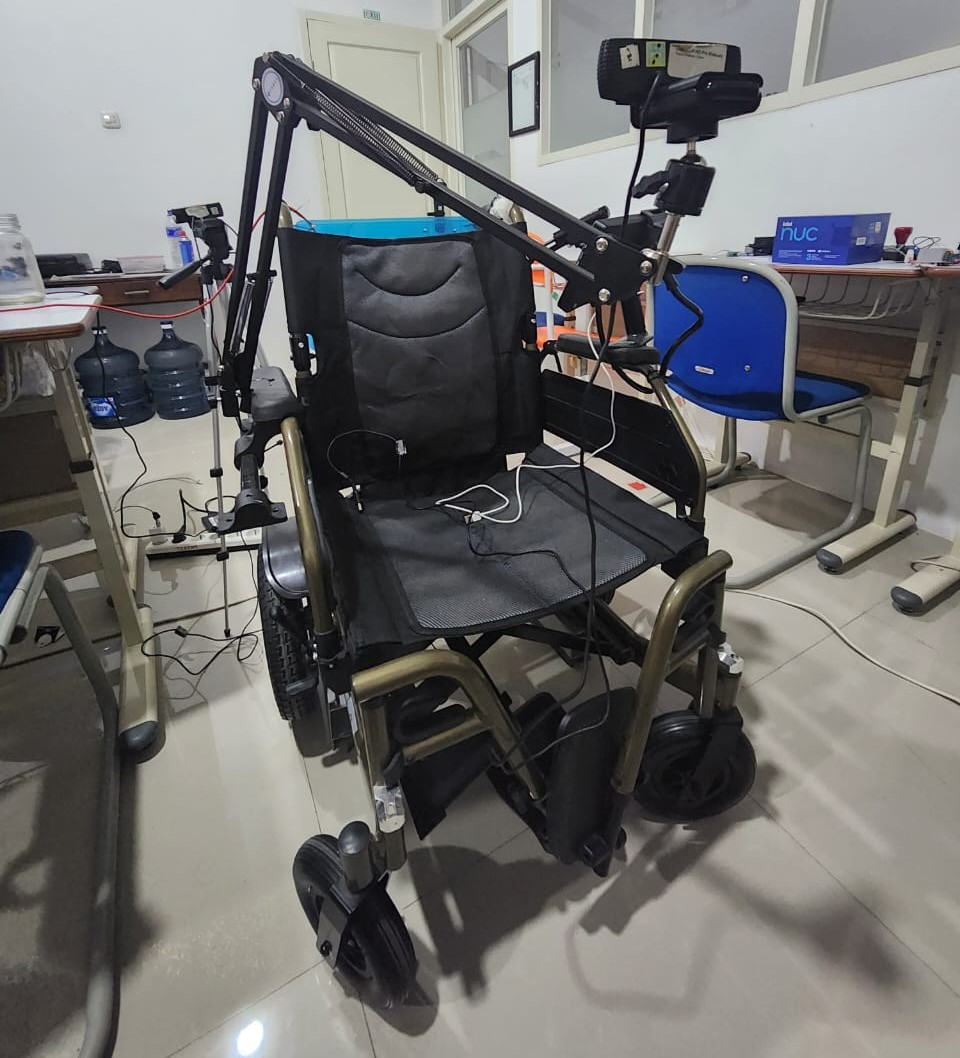
\includegraphics[width=.47\textwidth]{gambar/bab3/wheel.jpeg}

  % Ubah dengan keterangan gambar yang diinginkan
  \caption{Kursi Roda Elektrik}
  \label{fig:kursiroda}
\end{figure}

Kursi roda elektrik telah dikembangkan selama bertahun-tahun untuk digunakan oleh pasien dengan gangguan mobilitas di rumah dan masyarakat. Secara konvensional, lebih dari 80\% pengguna kursi roda elektrik mengoperasikan kursi rodanya dengan sebuah joystick sebagai antarmuka kendali. Joystick yang mendeteksi gerakan umumnya digunakan untuk mengoperasikan kursi roda elektrik. Selain itu, kecepatan kursi roda berubah seiring dengan jumlah defleksi dari joystick yang dilengkapi dengan pegas. Pengguna diharuskan menggunakan kendali proporsional dengan efisien untuk proprioception dan keterampilan sendi. Operasi yang tepat dari joystick memerlukan kontrol keterampilan motorik halus di tangan dan pergelangan tangan \parencite{koyama23}.



\section{\emph{Eye Gesture}}

\textit{Eye gesture} atau pose mata mengacu pada pergerakan mata, seperti tatapan mata, gerakan mata, dan ekspresi wajah, yang memainkan peran penting dalam komunikasi dan interaksi manusia \parencite{vanni_2022}. Perangkat pelacak mata telah digunakan untuk mempelajari berbagai aspek pose mata, termasuk pengaruh faktor sosial, faktor fisik, dan hubungan antara pose mata dan ucapan. Perangkat ini dapat merekam pose mata partisipan dengan kamera refleks kornea dan menganalisis gerakan tubuh dan pose mata dengan akurasi temporal\parencite{gullberg_kita_2009}. Contoh pose mata dapat dilihat pada Gambar \ref{fig:gaze}.

% Gambar 2.2
\begin{figure} [ht] \centering
    % Nama dari file gambar yang diinputkan
    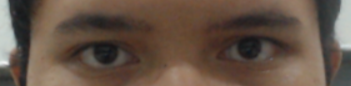
\includegraphics[width=.45\textwidth]{gambar/bab3/gaze.png}
    % Keterangan gambar yang diinputkan
    \caption{Pose Mata}
    % Label referensi dari gambar yang diinputkan
    \label{fig:gaze}
\end{figure}

Pose mata dapat digunakan dalam berbagai aplikasi, seperti kontrol komputer bebas genggam  dan gerakan yang menyertai ucapan. Sebagai contoh, teknik pelacakan tatapan mata untuk aplikasi interaktif, dengan fokus pada penggunaan pose mata sebagai alat kontrol \parencite{Morimoto_Mimica_2005}. 

\section{MediaPipe Face Mesh}

MediaPipe Face Mesh adalah solusi pendeteksi \textit{landmark} wajah yang memperkirakan 468 \textit{landmark} wajah 3D secara real-time, bahkan pada perangkat seluler. Solusi ini menggunakan \textit{pipeline} dari dua jaringan saraf untuk mengidentifikasi koordinat 3D landmark wajah dari gambar 2D. Jaringan pertama, BlazeFace, menghitung lokasi wajah dari gambar penuh, sementara jaringan kedua beroperasi pada wilayah yang dipotong untuk mengidentifikasi lokasi \textit{landmark} \parencite{mediapipe_2020}. Teknologi ini memiliki berbagai aplikasi, termasuk deteksi masker wajah, kontrol komputer bebas genggam, dan gerakan yang menyertai ucapan \parencite{thaman_2022}. Visualisasi dari MediaPipe Face Mesh dapat dilihat pada Gambar \ref{fig:facemesh}.

% Gambar 2.3
\begin{figure} [ht] \centering
    % Nama dari file gambar yang diinputkan
    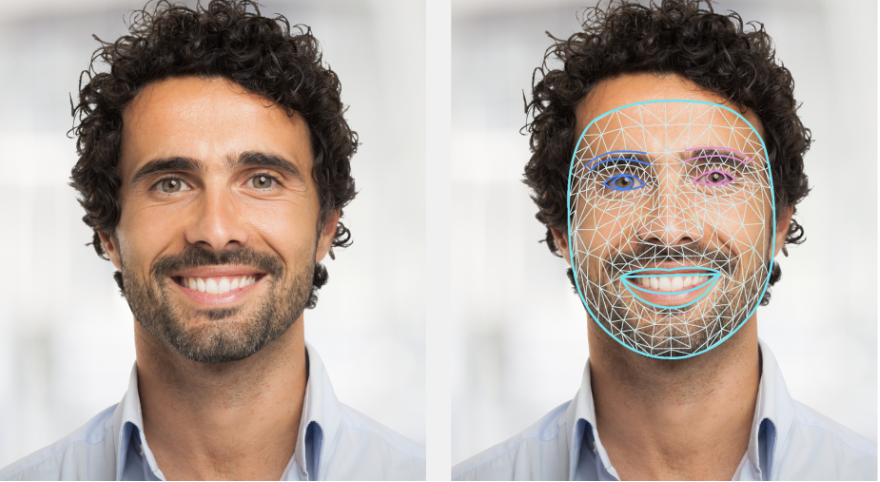
\includegraphics[width=.45\textwidth]{gambar/face_landmark.png}
    % Keterangan gambar yang diinputkan
    \caption{Visualisasi MediaPipe Face Mesh}
    % Label referensi dari gambar yang diinputkan
    \label{fig:facemesh}
\end{figure}

MediaPipe Face Mesh menyediakan antarmuka pemrograman yang sederhana, yang memungkinkan pengembang untuk mengakses koordinat \textit{landmark} di Python dan mengimplementasikan MediaPipe Face Mesh di berbagai aplikasi. Ini telah digunakan untuk deteksi \textit{landmark} wajah lintas platform secara \textit{real-time} dan dapat diintegrasikan ke dalam mesin grafis khusus untuk berbagai proyek \parencite{mediapipe_2020}. Model MediaPipe Face Mesh kompatibel dengan alat visualisasi MediaPipe dan dapat digunakan untuk membuat aplikasi untuk mendeteksi landmark wajah, ekspresi wajah, dan menerapkan filter dan efek wajah pada gambar dan video \parencite{Mediapipe_2023}.

Singkatnya, MediaPipe Face Mesh adalah alat yang ampuh untuk mendeteksi landmark wajah secara real-time, dengan berbagai aplikasi dalam visi komputer, interaksi manusia-komputer, dan \textit{augmented reality} (AR). Alat ini menawarkan antarmuka yang sederhana kepada para pengembang untuk mengakses dan memanfaatkan data \textit{landmark} wajah manusia untuk berbagai tujuan inovatif.

\section{\emph{Convolutional Neural Network} (CNN)}

\emph{Convolutional Neural Network} (CNN) adalah jenis jaringan syaraf tiruan yang digunakan terutama untuk pengenalan dan pemrosesan gambar. Ini adalah bagian dari pembelajaran mesin dan dirancang khusus untuk mengidentifikasi dan mengenali objek dalam gambar, serta untuk tugas-tugas seperti klasifikasi objek dan pengenalan pola \parencite{arm_2023}. CNN dicirikan oleh kemampuannya untuk mempelajari rekayasa fitur dengan sendirinya melalui pengoptimalan filter, dan mereka mencegah masalah seperti gradien yang menghilang dan gradien yang meledak, yang terlihat pada jaringan saraf sebelumnya, dengan menggunakan bobot yang diatur melalui koneksi yang lebih sedikit. 

Arsitektur CNN dianalogikan dengan pola konektivitas otak manusia, dengan neuron yang disusun dengan cara tertentu untuk memproses rangsangan visual, dan terdiri dari lapisan-lapisan seperti lapisan konvolusi, lapisan penyatuan, dan lapisan yang terhubung sepenuhnya \parencite{ibm_2023}. CNN memiliki berbagai macam aplikasi, termasuk klasifikasi gambar, pemrosesan bahasa alami, dan estimasi kedalaman untuk mobil swakemudi \parencite{arm_2023}.

Arsitektur pada CNN terdiri dari tiga bagian, yaitu input, \emph{feature learning}, dan \emph{classification}. \emph{Feature Learning} terdiri dari dua buah \emph{convolution layer} dan dua buah \emph{pooling layer}. Pada \emph{classification} terdiri dari dua \emph{hidden layer} dan satu \emph{output layer}. Arsitektur CNN dapat digambarkan seperti pada Gambar \ref{fig:arsitektur cnn}.

% Gambar 2.4
\begin{figure} [ht] \centering
    % Nama dari file gambar yang diinputkan
    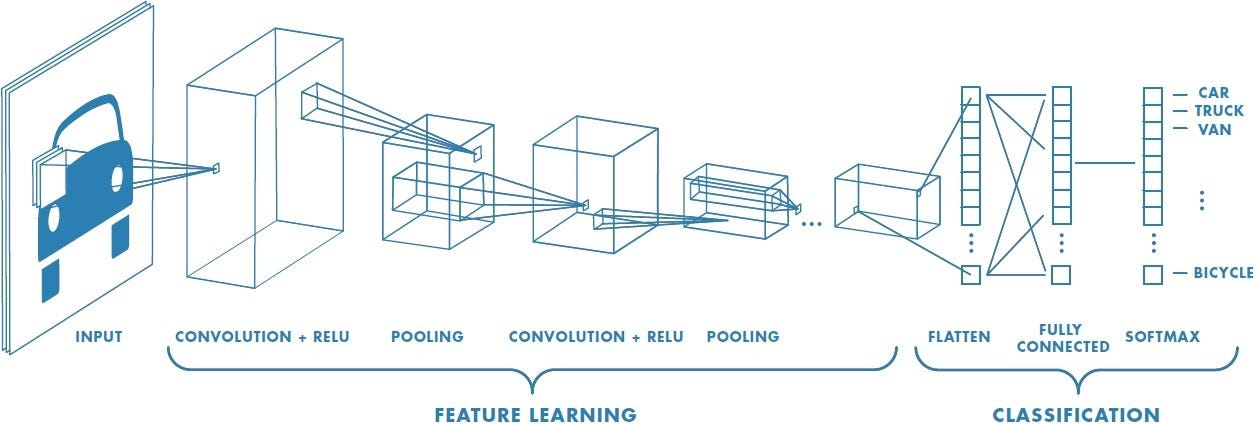
\includegraphics[width=1\textwidth]{gambar/cnn.jpg}
    % Keterangan gambar yang diinputkan
    \caption{Arsitektur \emph{Convolutional Neural Network}}
    % Label referensi dari gambar yang diinputkan
    \label{fig:arsitektur cnn}
\end{figure}

Input CNN merupakan array tiga dimensi dengan ukuran seperti pada Persamaan \ref{eq:cnn}. Apabila input merupakan suatu citra maka citra tersebut harus diubah menjadi array dua dimensi. 

% Persamaan 2.1
\begin{equation}
\label{eq:cnn}
Baris * Kolom * Depth
\end{equation}

\emph{Convolution Layer} digunakan untuk menyaring (\emph{filter}) matriks dari citra \emph{input}. \emph{Zero Padd-ing} akan diperlukan untuk mempertahankan ukuran matriks dari citra \parencite{dwitama2019klasifikasi}. Ukuran kernel yang digunakan pada layer konvolusi adalah \(3 \times 3\) dan \(5 \times 5\). \emph{Output} dari lapisan konvolusi ini akan digunakan sebagai \emph{input} pada \emph{Pooling Layer} \parencite{hakim2018penerapan}. Apabila output dari \emph{Convolution Layer} bernilai negatif maka akan dilakukan perhitungan tambahan berupa aktifasi ReLU. Fungsi aktivasi ReLU akan nilai matriks yang bernilai negatif menjadi nol. Contoh penerapan dari aktivasi ReLU dapat dilihat pada Gambar \ref{fig:Aktivasi ReLU}.

% Gambar 2.5
\begin{figure} [ht] \centering
    % Nama dari file gambar yang diinputkan
    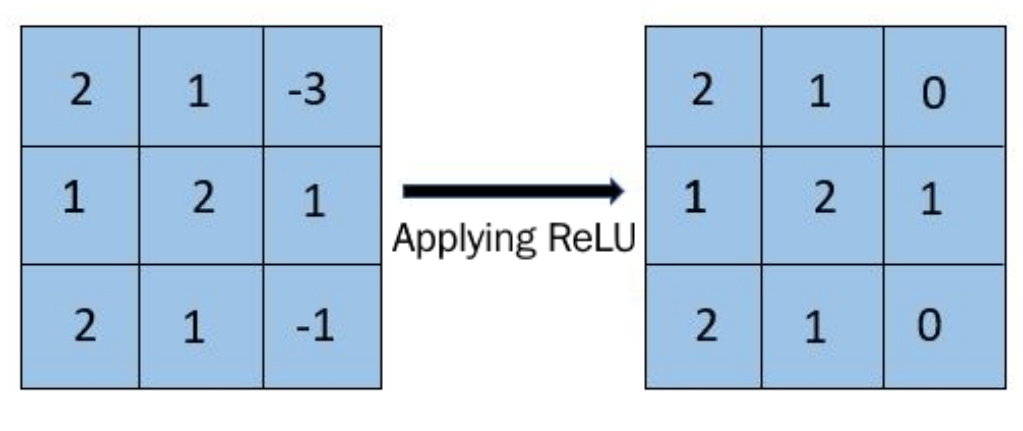
\includegraphics[width=.6\textwidth]{gambar/relu.png}
    % Keterangan gambar yang diinputkan
    \caption{\emph{Aktivasi ReLU}}
    % Label referensi dari gambar yang diinputkan
    \label{fig:Aktivasi ReLU}
\end{figure}

\emph{Pooling Layer} digunakan untuk mengurangi jumlah parameter ketika ukuran citra terlalu besar dengan cara mengurangi dimensi setiap fitur. Karena ukuran citra menjadi lebih kecil maka proses \emph{feature map} akan menjadi lebih cepat \parencite{hakim2018penerapan}. \emph{Max Pooling} dilakukan dengan cara mengambil nilai dengan elemen terbesar sesuai dengan ukuran filter. Sebagai contoh pada Gambar \ref{fig:Max Pooling} merupakan \emph{max pooling} dengan filter \(2 \times 2\) dengan \emph{stride} sebesar 2.

% Gambar 2.6
\begin{figure} [ht] \centering
    % Nama dari file gambar yang diinputkan
    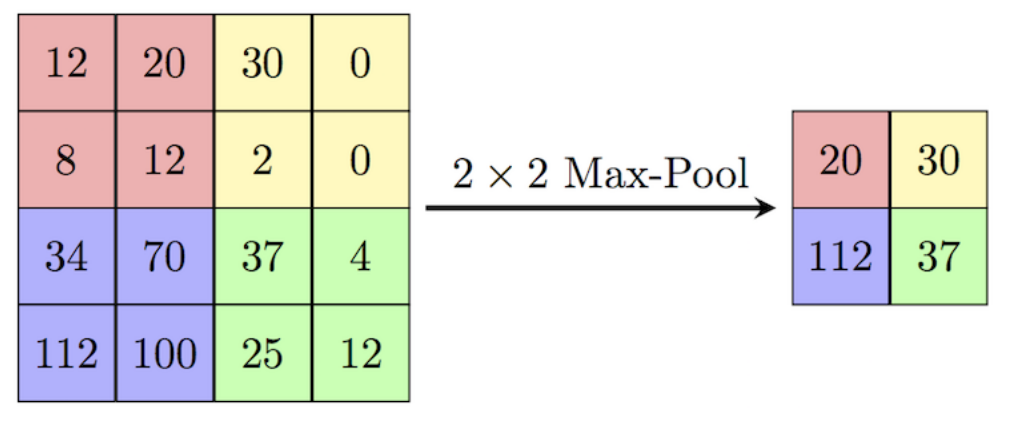
\includegraphics[width=.6\textwidth]{gambar/pooling.png}
    % Keterangan gambar yang diinputkan
    \caption{\emph{Max Pooling}}
    % Label referensi dari gambar yang diinputkan
    \label{fig:Max Pooling}
\end{figure}

Dalam \textit{feature learning}, data yang umumnya berbentuk multi-dimensi (seperti gambar yang memiliki lebar, tinggi, dan kedalaman warna) diproses melalui lapisan-lapisan untuk menghasilkan fitur yang lebih abstrak dan representatif. Namun, lapisan selanjutnya dalam jaringan saraf, yaitu lapisan \textit{fully connected} atau lapisan yang sepenuhnya terhubung, memerlukan input berbentuk vektor satu dimensi.

Proses \textit{Flatten} berfungsi untuk mengubah output multi-dimensi dari \textit{feature learning} menjadi vektor satu dimensi. Caranya adalah dengan mengatur ulang seluruh elemen matriks hasil \textit{feature learning} menjadi sebuah barisan panjang elemen-elemen. Proses ini memastikan bahwa semua informasi yang diperoleh dari \textit{feature learning} dapat diproses secara efektif dalam lapisan klasifikasi, memungkinkan jaringan untuk membuat keputusan atau prediksi berdasarkan fitur yang telah dipelajari. Flatten dapat digambarkan seperti pada Gambar \ref{fig:Proses Flattening}.

% Gambar 2.7
\begin{figure} [ht] \centering
    % Nama dari file gambar yang diinputkan
    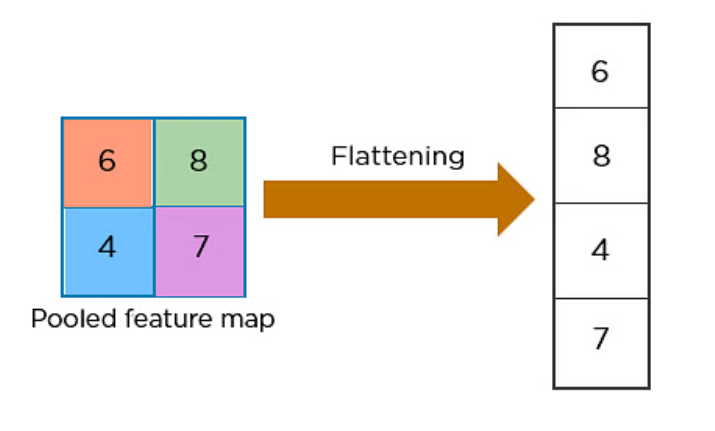
\includegraphics[width=.6\textwidth]{gambar/flatten.png}
    % Keterangan gambar yang diinputkan
    \caption{Proses \emph{Flattening}}
    % Label referensi dari gambar yang diinputkan
    \label{fig:Proses Flattening}
\end{figure}

%\newpage

\section{Matriks Performa Klasifikasi}

\emph{Confusion Matrix} adalah alat yang digunakan untuk mengevaluasi kinerja model klasifikasi dalam pembelajaran mesin. Tabel ini memberikan gambaran mendetail tentang bagaimana model klasifikasi bekerja, menunjukkan hubungan antara prediksi model dengan nilai sebenarnya. \emph{Confusion Matrix} adalah representasi tabel yang terdiri dari empat komponen utama, yaitu \emph{True Positive} (TP), \emph{False Positive} (FP), \emph{True Negative} (TN), dan \emph{False Negative} (FN). Setiap komponen memiliki makna yang spesifik dalam konteks prediksi \parencite{provost2013data}. Visualisasi \emph{confusion matrix} dapat dilihat pada Gambar \ref{fig:confusion}. 

% Gambar 2.7
\begin{figure} [ht] \centering
    % Nama dari file gambar yang diinputkan
    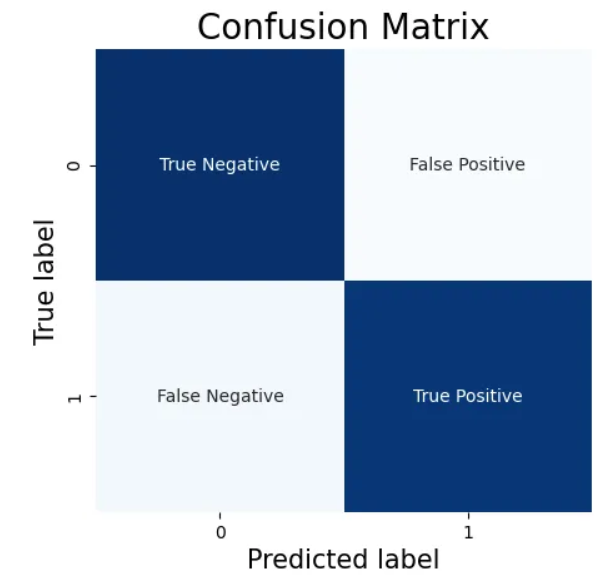
\includegraphics[width=.4\textwidth]{gambar/bab2/confusion.png}
    % Keterangan gambar yang diinputkan
    \caption{Visualisasi \emph{confusion matrix}}
    % Label referensi dari gambar yang diinputkan
    \label{fig:confusion}
\end{figure}

True Positive (TP) adalah prediksi benar terhadap kelas positif. Sebagai contoh, model memprediksi bahwa pasien menderita penyakit tertentu, dan pasien tersebut benar-benar memiliki penyakit tersebut. False Positive (FP), juga dikenal sebagai "Type I Error," adalah prediksi salah terhadap kelas positif. Contohnya adalah ketika model memprediksi bahwa pasien memiliki penyakit tertentu, tetapi sebenarnya pasien tersebut sehat. True Negative (TN) adalah prediksi benar terhadap kelas negatif, yaitu ketika model memprediksi bahwa pasien sehat, dan pasien tersebut benar-benar sehat. False Negative (FN), atau "Type II Error," adalah prediksi salah terhadap kelas negatif, di mana model memprediksi bahwa pasien sehat, tetapi sebenarnya pasien tersebut memiliki penyakit tertentu. 

Untuk memahami bagaimana model klasifikasi bekerja, kita perlu memahami beberapa metrik evaluasi kinerja berdasarkan \emph{Confusion Matrix}. Metrik evaluasi kinerja terdiri dari \emph{Accuracy}, \emph{Precision}, \emph{Recall}, dan \emph{F-1 Score}. Metrik ini memberikan informasi yang berguna tentang seberapa baik model klasifikasi bekerja dalam memprediksi kelas target \parencite{provost2013data}.

\subsection{\emph{Accuracy}}
\label{subsec:acc_klasifikasi}

\emph{Accuracy} adalah ukuran kinerja yang menunjukkan seberapa tepat model dapat mengklasifikasikan data uji secara benar. Dalam konteks ini, akurasi adalah rasio antara prediksi yang benar (TP dan TN) dengan total jumlah data. Dengan kata lain, akurasi mengukur seberapa dekat nilai prediksi dengan nilai aktual. Nilai \emph{accuracy} dapat diperoleh menggunakan Persamaan \ref{eq:acc}. 

\begin{equation}
  \label{eq:acc}
  Accuracy=\frac{TP+TN}{TP+TN+FP+FN}
\end{equation}

\subsection{\emph{Precision}}
\label{subsec:prec_klasifikasi}

\emph{Precision} adalah ukuran kinerja yang menunjukkan tingkat keakuratan data yang diminta dibandingkan dengan hasil prediksi yang diberikan oleh model. Dalam konteks ini, presisi adalah rasio antara prediksi positif yang benar (TP) dengan total hasil prediksi positif (TP dan FP). Nilai \emph{precision} dapat diperoleh dengan Persamaan \ref{eq:prec}.

\begin{equation}
  \label{eq:prec}
  Precision=\frac{TP}{TP+FP}
\end{equation}

\subsection{\emph{Recall}}
\label{subsec:recall_klasifikasi}

\emph{Recall} adalah ukuran kinerja yang menunjukkan seberapa berhasil model dalam menemukan kembali suatu informasi. Dalam konteks ini, recall adalah rasio antara prediksi positif yang benar (TP) dengan total jumlah data aktual positif (TP dan FN). Dengan demikian, nilai recall dapat dihitung menggunakan Persamaan \ref{eq:recall}.

\begin{equation}
  \label{eq:recall}
  Recall=\frac{TP}{TP+FN}
\end{equation}

\subsection{\emph{F1-Score}}
\label{subsec:score_klasifikasi}

\emph{F1-Score} adalah nilai antara nol (0) hingga satu (1) yang diperoleh dari rata-rata harmonis (\emph{harmonic mean}) antara nilai \emph{precision} dan nilai \emph{recall}. Oleh karena itu, nilai \emph{F1-Score} dapat dihitung menggunakan Persamaan \ref{eq:score}.

\begin{equation}
  \label{eq:score}
  F{1}{-}Score=\frac{2 \times Precision \times Recall}{Precision+Recall}
\end{equation}

Kesimpulannya adalah \emph{accuracy} mengukur seberapa sering model membuat prediksi yang benar dari keseluruhan prediksi. \emph{Precision} menilai seberapa banyak prediksi positif yang benar-benar positif. \emph{Recall} mengukur seberapa baik model dalam menangkap semua kasus positif yang sebenarnya. \emph{F1-score} memberikan keseimbangan antara presisi dan recall, yang berguna ketika kita membutuhkan keseimbangan antara kedua metrik tersebut. Dengan menggunakan metrik ini, model dapat dievaluasi dan ditingkatkan sesuai dengan kebutuhan.

\section{\emph{Pulse Width Modulation} (PWM)}

\emph{Pulse Width Modulation} (PWM) adalah metode pengaturan sinyal digital yang digunakan untuk mengontrol daya yang disediakan ke perangkat elektronik. PWM menghasilkan sinyal pulsa dengan lebar pulsa yang dapat diatur, yang memungkinkan pengontrolan daya yang diberikan ke perangkat. PWM digunakan dalam berbagai aplikasi, termasuk pengendalian motor, pengendalian lampu, dan pengendalian suhu. PWM bekerja dengan menghasilkan sinyal pulsa dengan lebar pulsa yang dapat diatur, yang kemudian diubah menjadi sinyal analog dengan menggunakan filter. Pada Gambar \ref{fig:pwm} merupakan contoh PWM dalam induktor ideal yang digerakkan oleh sumber tegangan yang dimodulasi sebagai serangkaian pulsa (-V), menghasilkan arus seperti sinusoidal dalam induktor (-B). Pulsa tegangan persegi panjang tetap menghasilkan bentuk gelombang arus yang semakin halus, seiring dengan meningkatnya frekuensi pengalihan. Bentuk gelombang arus adalah integral dari bentuk gelombang tegangan. 

\begin{figure} [ht] \centering
  % Nama dari file gambar yang diinputkan
  \includegraphics[scale=0.4]{gambar/pwm.png}
  % Keterangan gambar yang diinputkan
  \caption{Visualisasi PWM}
  % Label referensi dari gambar yang diinputkan
  \label{fig:pwm}
\end{figure}

PWM memiliki beberapa keuntungan dibandingkan dengan metode pengaturan daya lainnya, seperti pengaturan tegangan atau arus. Salah satu keuntungan utama dari PWM adalah efisiensi energi yang lebih tinggi, karena daya yang disediakan ke perangkat hanya diatur dengan mengubah lebar pulsa sinyal, bukan dengan mengubah tegangan atau arus. Selain itu, PWM juga memungkinkan pengontrolan daya yang lebih halus dan presisi, karena lebar pulsa sinyal dapat diatur dalam rentang yang sangat luas. PWM juga dapat digunakan untuk mengontrol kecepatan motor DC, mengatur kecerahan lampu LED, dan mengontrol suhu dalam sistem pemanas dan pendingin.

Dalam aplikasi ini, PWM digunakan untuk mengontrol kecepatan motor DC pada kursi roda elektrik. Dengan menggunakan PWM, kecepatan motor dapat diatur dengan presisi, sehingga pengguna dapat mengontrol kursi roda dengan lebih mudah dan nyaman. PWM juga memungkinkan pengguna untuk mengatur kecepatan motor sesuai dengan kebutuhan, sehingga kursi roda dapat bergerak dengan lancar dan stabil. Dengan menggunakan PWM, kursi roda dapat bergerak dengan lebih efisien dan efektif, sehingga pengguna dapat menggunakannya dengan lebih nyaman dan aman. Nilai PWM yang digunakan dalam penelitian ini terdapat 2 yaitu, \emph{turn speed} sebesar 40 pwm atau 15 rpm dan \emph{max speed} sebesar 80 pwm atau 32 rpm.

\section{ESP32 DevKit V1}

ESP32 DevKit V1 pertama kali dirilis oleh Espressif Systems pada tahun 2016. ESP32, sebagai penerus dari ESP8266, diperkenalkan dengan berbagai peningkatan fitur dan performa yang signifikan. ESP32 DevKit V1 adalah modul pengembangan berbasis mikrokontroler ESP32 yang dirancang oleh Espressif Systems. Modul ini sangat populer di kalangan pengembang \emph{Internet of Things} (IoT) karena kinerjanya yang tinggi dan fiturnya yang kaya. ESP32 DevKit V1 memiliki prosesor dual-core dengan kecepatan hingga 240 MHz, memberikan kemampuan pemrosesan yang tinggi untuk aplikasi yang membutuhkan performa tinggi. Modul ini dilengkapi dengan konektivitas Wi-Fi 802.11 b/g/n dan Bluetooth 4.2, memungkinkan berbagai jenis komunikasi nirkabel dalam satu perangkat. Dengan RAM 520 KB dan penyimpanan flash eksternal yang bervariasi, biasanya antara 4 MB dan 16 MB, modul ini cukup memadai untuk menjalankan aplikasi yang kompleks. ESP32 Devkit V1 dapat dilihat pada Gambar \ref{fig:esp32}.

\begin{figure} [ht] \centering
  % Nama dari file gambar yang diinputkan
  \includegraphics[scale=0.2]{gambar/esp32.jpg}
  % Keterangan gambar yang diinputkan
  \caption{ESP32 Devkit V1}
  % Label referensi dari gambar yang diinputkan
  \label{fig:esp32}
\end{figure}

Selain itu, ESP32 DevKit V1 memiliki banyak pin GPIO yang dapat diprogram untuk berbagai fungsi seperti PWM, ADC, DAC, UART, SPI, dan I2C, sehingga memberikan fleksibilitas yang tinggi dalam berinteraksi dengan berbagai sensor dan aktuator. Modul ini juga dilengkapi dengan sensor suhu internal dan sensor efek hall yang dapat digunakan untuk berbagai aplikasi sensor. Dalam hal efisiensi energi, ESP32 mendukung berbagai mode hemat energi seperti \emph{deep sleep} dan \emph{light sleep}, yang sangat berguna untuk aplikasi yang bergantung pada baterai.

ESP32 DevKit V1 sering digunakan dalam berbagai proyek IoT, seperti \emph{smart home}, \emph{monitoring} lingkungan, proyek robotika, dan sistem keamanan. Modul ini dapat diprogram menggunakan berbagai lingkungan pengembangan, termasuk Arduino IDE, PlatformIO, dan Espressif IoT Development Framework (ESP-IDF). Dengan fitur yang kaya, dukungan komunitas yang luas, dan kemampuan pemrograman yang fleksibel, ESP32 DevKit V1 adalah pilihan yang sangat baik bagi pengembang yang ingin membangun perangkat IoT yang efisien. Dalam penelitian ini, selain sebagai \emph{controller} kursi roda, ESP32 Devkit V1 juga digunakan sebagai \emph{Access Point}, yang memungkinkan perangkat lain dapat terhubung ke jaringan Wi-Fi lokal yang dibentuk oleh ESP32, untuk menerima data dari perangkat lain.

\section{\textit{Next Unit of Computing} (NUC)}

Pada tahun 2012, Intel meluncurkan arsitektur \textit{Next Unit of Computing}, yang disebut dengan konsep "NUC", yang sebenarnya adalah \textit{mini quasi-system PC}. Intel Hades Canyon NUC generasi pertama mengungguli semua PC mini lainnya dengan ukuran tablet 7 inci. Performa yang kuat, berbagai antarmuka dan desain penampilan yang luar biasa adalah unik di hadapan produk dari berbagai OEM, bahkan lebih baik daripada Mac mini\parencite{8858650}. NUC dapat dilihat pada Gambar \ref{fig:Perangkat NUC}.

% Gambar 2.8
\begin{figure} [ht] \centering
    % Nama dari file gambar yang diinputkan
    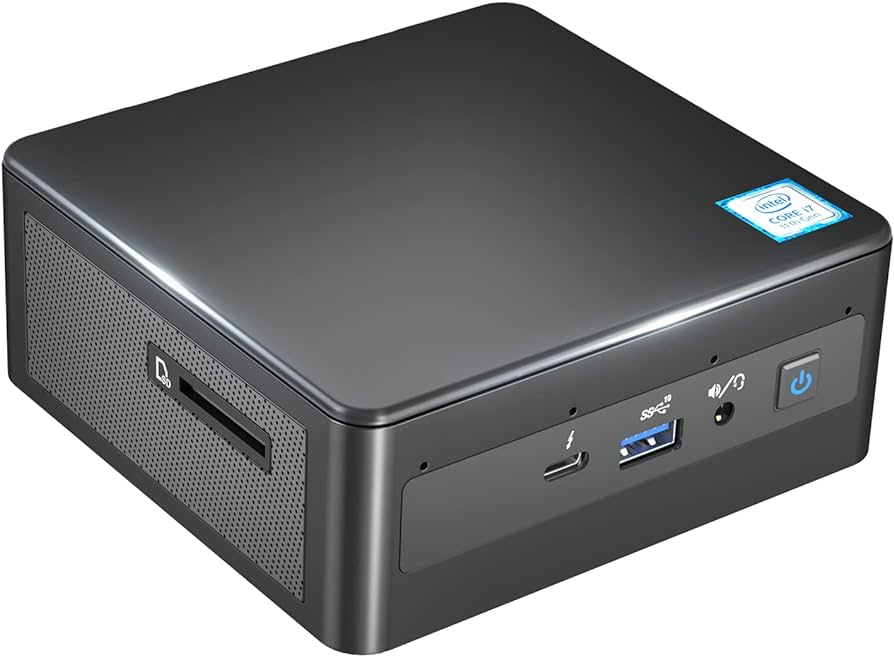
\includegraphics[scale=0.2]{gambar/nuc.jpg}
    % Keterangan gambar yang diinputkan
    \caption{Perangkat NUC}
    % Label referensi dari gambar yang diinputkan
    \label{fig:Perangkat NUC}
\end{figure}

Selama bertahun-tahun, dibatasi oleh ukurannya yang kecil, NUC hanya dapat menggunakan kartu grafis inti Intel, yang tertinggal di belakang kartu grafis eksternal, bahkan lebih rendah dari AMD APU. Pada tahun 2017, Intel dan AMD mulai mengembangkan chip hybrid. Pada tahun 2018, chip hybrid Intel pada awalnya dibentuk dan lima produk pertama diumumkan, termasuk i7-8809G. Prosesor Intel, yang mengintegrasikan prosesor grafis AMD RX Vega, merupakan bagian dari seri Kaby Lake-G, sehingga Intel dapat menutupi kekurangannya dalam kinerja GPU\parencite{8858650}.

Pada penelitian ini digunakan Intel NUC 11 Pro Performance Kit dengan versi NUC11PAHi7 memiliki prosesor Intel Core i7-1165G7 generasi ke-11. Prosesor ini memiliki kecepatan dasar sebesar 2,8 GHz dan dapat mencapai kecepatan boost hingga 4,7 GHz. Selain itu, terdapat Intel Iris Xe Graphics yang memungkinkan perangkat untuk menjalankan berbagai aplikasi berbasis GPU dengan lancar. Dilengkapi dengan 2 buah 16 GB RAM DDR4 (32 GB) dan 256 GB SSD PCIe M.2. Mendukung hingga 4 monitor melalui HDMI, mini DP, dan 2 port Thunderbolt (memerlukan adaptor). Resolusi maksimum monitor dapat mencapai 4K (3840x2160). Serta fitur-fitur lainnya seperti Wi-Fi 6 AX201, Bluetooth 5.2, Ethernet LAN (RJ-45), dan jack headset stereo depan.